\documentclass[addpoints]{exam}

\usepackage{graphicx}
\usepackage{hyperref}
\usepackage{tabularx}

\graphicspath{{images/}}

% Header and footer.
\pagestyle{headandfoot}
\runningheadrule
\runningfootrule
\runningheader{CS 440}{HW III: WebGL}{Fall 2020}
\runningfooter{}{Page \thepage\ of \numpages}{}
\firstpageheader{}{}{}

\qformat{{\large\bf \thequestion. \thequestiontitle}\hfill[\totalpoints\ points]}
\boxedpoints

\title{Homework III: WebGL}
\author{CS 440 Computer Graphics\\Habib University\\Fall 2020}
\date{Due: 18h on Monday, 12 October}

\begin{document}
\maketitle

Each problem below specifies the names of the files you have to submit for it. Please make sure your submitted files have the indicated names. Any files in your GitHub repository with these names at the time of the deadline will be considered as your submission.

\begin{questions}

  \titledquestion{Geometry trumps JS}[0]

  We will be using WebGL to render 3D geometry in the browser. Programming for WebGL is done in JavaScript which is not natively aware of geometric types, e.g. vector. The file, \texttt{MV.js}, in the \texttt{Common} folder in the \texttt{Code} section on the \href{https://www.cs.unm.edu/~angel/BOOK/INTERACTIVE_COMPUTER_GRAPHICS/SEVENTH_EDITION/}{website of this module's book} defines abstractions that allow programs to be written in terms of geometric entities, e.g. a vector instead of JavaScript array. It also defines a function to convert these types to the required JavaScript types when needed. 

  Go over the file {\tt MV.js} in order to get familiar with the types that it provides and their related operations. Especially note how the \texttt{mix} function can be used for interpolaton.

  You need not spend too much time understanding the function bodies as long as you can infer, e.g. from its name, what the function does. For now, you may skip the functions in the following sections in the file.
  \begin{itemize}
  \item ModelView Matrix Generators, and
  \item Projection Matrix Generators.
  \end{itemize}

  Wherever possible in your code for subsequent problems, prefer using geometric primitives and operations from {\tt MV.js} over those provided natively by JavaScript. For this, your files may include the \texttt{MV.js} file over the web.

\titledquestion{Mandelbrot Revisited}[10]

  Visualize the Mandelbrot set from HW 2. Set the threshold value, $n_t$, for the visualization either through interactive user input or as a global variable at the top of your JS file.
  
  \noindent\underline{Files}: \texttt{mandelbrot.html, mandelbrot.js}
  
  \titledquestion{Maxwell's Triangle}[5]
  \label{q:maxwell}
  
  \begin{tabularx}{\linewidth}{cX}
    \raisebox{-\totalheight}{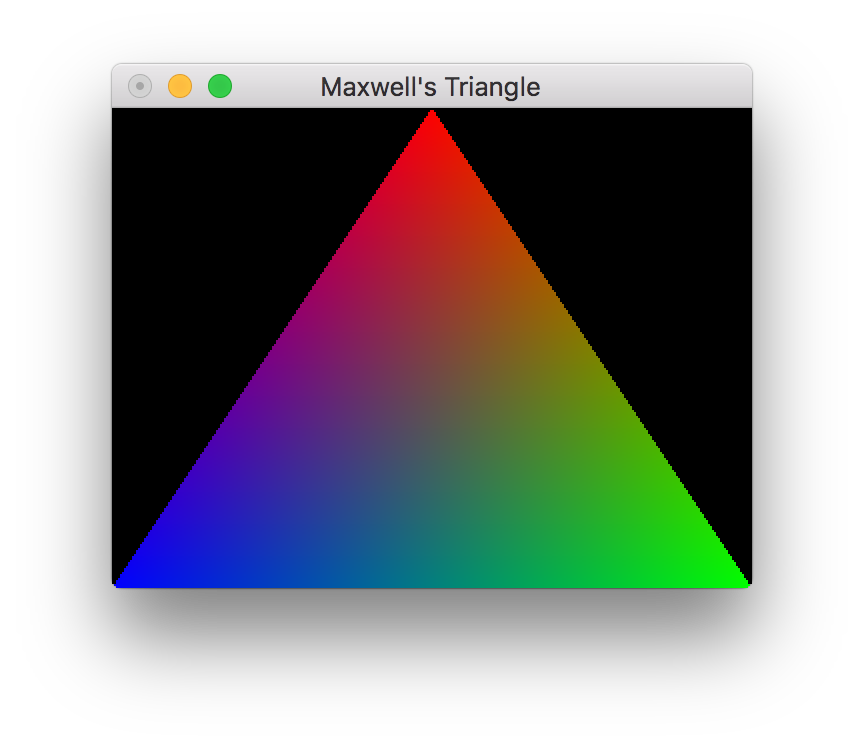
\includegraphics[width=.35\linewidth]{maxwell}}
    &
    \href{https://en.wikipedia.org/wiki/James_Clerk_Maxwell}{James Clerk Maxwell} is best known for his work in electromagnetic radiation resulting in the well known \href{https://en.wikipedia.org/wiki/Maxwell\%27s_equations}{Maxwell's equations}.
    
    Not surprisingly, he was also among the first ones to explore the \href{https://spie.org/publications/pm105_32_maxwell_triangle?SSO=1}{trichromatic theory of color}. This has led to what is now known as \href{https://homepages.abdn.ac.uk/npmuseum/article/Maxwell/Legacy/MaxTri.html}{Maxwell's triangle}, simply called the \href{https://en.wikipedia.org/wiki/Color_triangle}{color triangle}. It is a triangle with the primary colors at its vertices and its interior shaded by linear combinations of the colors at the vertices. At any interior point, the amount of color contributed by a vertex is proportional to the distance of the vertex from that point.
  \end{tabularx}

  WebGL interpolates the colors of the vertices across the primitve by default, similar to your line and polygon fuinctions from HW 2. Use this property to display Maxwell's triangle: a triangle whose vertices are red, green, and blue.
  
  \underline{Files}: \texttt{maxwell.html, maxwell.js}
  
  \titledquestion{Colors}[15]

  Write a program that displays a triangle along with its boundary edges which may be colored differently than the triangle. The user is presented on the main page with the following interactive rendering options.
  \begin{itemize}
  \item Set the RGB colors of the boundary vertices.
  \item Set the RGB colors of the triangle (interior) vertices.
  \item The display of the boundary can be toggled on or off.
  \item The display of the interior can be toggled on or off.
  \item Each of the boundary and interior vertices can be assigned a random RGB color.
  \end{itemize}

  \noindent\underline{Files}: {\tt colors.html, colors.js}

  \titledquestion{Tetrix}[15]

  \begin{tabular}{ccc}
    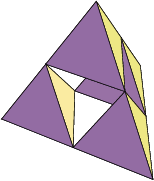
\includegraphics[width=.3\textwidth]{tetrix1}
    & 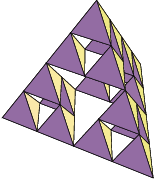
\includegraphics[width=.3\textwidth]{tetrix2}
    & 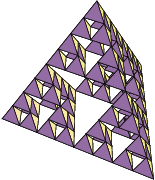
\includegraphics[width=.3\textwidth]{tetrix3}
  \end{tabular}
  A \href{http://mathworld.wolfram.com/Tetrix.html}{\it tetrix} is the 3D version of the Sierpinski triangle and is also referred to as the \textit{Sierpinski tetrahedron}. Write a program to render a tetrix at a specified recursion level. The rendered tetrix should be animated to be continuously rotating about an axis and the user should be able to toggle between rotation about the x, y, or z axis. The recursion level is to be specified through a slider with appropriate bounds and should take effect immediately.

  \noindent\underline{Files}: {\tt tetrix.html, tetrix.js}

  \titledquestion{Polygons Galore}[15]
  \label{q:galore}
  
  \begin{tabularx}{\linewidth}{lX}
    \raisebox{-.9\totalheight}{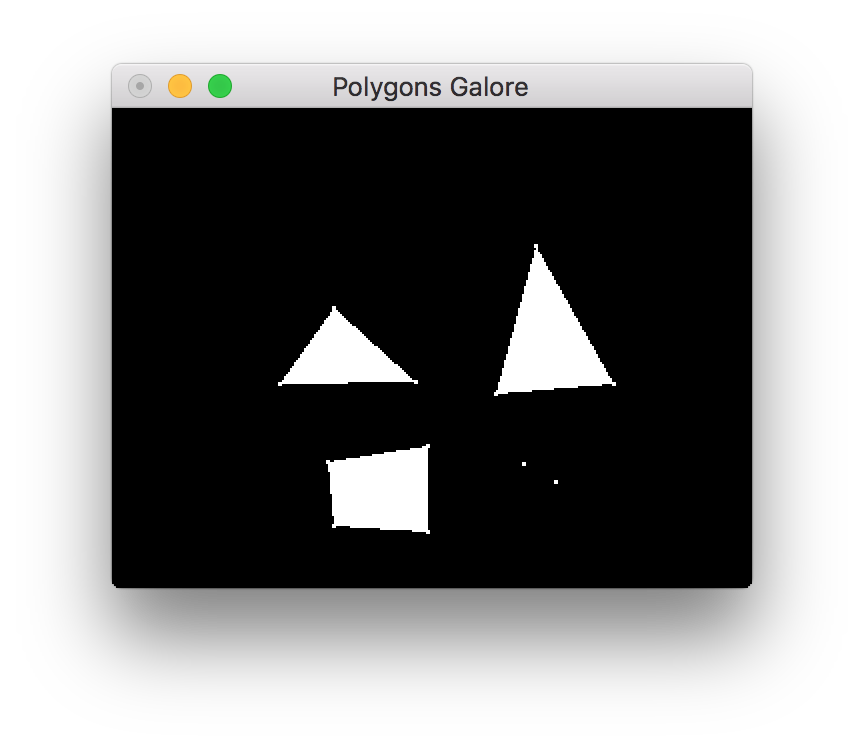
\includegraphics[width=.35\textwidth]{galore}}
    &
    Write a program that interactively draws triangles and quadrilaterals. The user indicates the vertices by clicking in the canvas, i.e. the position of the click is registered as a vertex. The program supports two {\it modes}--triangle mode (default) and quad mode. In triangle mode, every 3 consecutive vertices are drawn as a triangle. In quad mode, every 4 consecutive vertices are drawn as a quadrilateral. Vertices that are not yet part of a polygon are drawn as points. Each drawn shape is assigned a different random color. Furthermore, the following interaction is supported.
  \end{tabularx}
    \begin{parts}
    \part Pressing \texttt{r} or \texttt{R} resets to default. That is, the canvas is cleared and the drawing mode is set to triangle mode.
    \part Pressing \texttt{t} or \texttt{T} toggles between the drawing modes. Vertices that have not yet completed a polygon at the time of the toggle should be handled according to the new mode, they should not be discarded. Polygons drawn before the toggle should not be affected.
  \end{parts}
  \noindent\underline{Files}: {\tt galore.html, galore.js}

    \titledquestion{Reflex Game}[20]

      Write a game to test the player's reflexes. The player has to click on a polygon that appears for a brief period at a random location in the canvas. After a fixed interval the polygon disappears and reappears at another location. If the players is able to click inside the polygon before it disappears, her score increments, and the polygon disappears to reappear at another location. If she clicks on a blank location, e.g. the polygon there has already disappeared, her score decrements. If she has not clicked at all for three consecutive polygons, her score decrements. The player starts the game with a score of 0 and the game ends when her score becomes negative.
      
  \underline{Files}: {\tt reflex.html, reflex.js}

    \titledquestion{Random Time Waste}[0]
  
  If you find youeself with time to kill, you can make the reflex game more interesting by implementing the following features.
  \begin{parts}
    \part Appearance: the shape and color of the polygon change between appearances.
    \part Score: the current score is displayed and updated on the page.
    \part Game speed: the duration of the polygon's appearance on screen is adaptive. It decreases as the player's score increases and increases if the player loses score due to wrong clicks or lack of clicks.
    \part Time: a timer appears on the page that counts down from 30 seconds. The game ends as before or when the timer reaches 0.
  \end{parts}
  Your main page should clearly indicate any implemented features, whether from above or otherwise, for the benefit of your reviewer. Note that your reviewer may not be as blessed with time as yourself and may not review this question. It carries 0 points.
      
  \underline{Files}: {\tt wasteoftime.html, wasteoftime.js}
  
\end{questions}

\end{document}
%%% Local Variables:
%%% mode: latex
%%% TeX-master: t
%%% End:
